\chapter{Previous Work on Attribute Level Sets}
\label{sec:prev}
In this section, previous work on attribute level sets on neuronal models is described. The contents of this section are mainly based on \cite{Oly,Rot,Iii2019}. 
\section{Existence of attribute level sets in complex systems}
Contribution in \cite{Oly} focus on proving the existence of attribute level sets in complex neuronal systems and networks, although results are more general and could be applied to any model based on parameters meeting certain specific requirements.

The technique is mainly based on the implicit function theorem which imposes certain conditions which need to be guaranteed. For instance, the method developed can only applied to first-order differentiable (on variables and parameters) models.

Using the implicit functions theorem, they are able not only to prove the existence of attribute level sets near a generic point on parameter space, but also to compute the exact compensatory function (attribute level sets) on parameter space, using the linear approximation also provided by the theorem. They propose an algorithm to compute exact compensatory covariations.

Moreover the algorithm developed was applied to a biophysical conductance-based model, consisting in two identical neurons that mutually inhibit one another. Two attribute level sets were computed on different parameter spaces in order to illustrate the method.

On the one hand, they considered the $\bar{g}_{h}-\bar{g}_{SynS}$ parameter space. Here, $\bar{g}_{h}$ is the maximal conductance of a hyperpolarization-activated current ($I_{h}$) and $\bar{g}_{SynS}$ the maximal conductance of the chemical synapses current. They found level sets on this parameter space preserving the burst period (T). Bursting is characterized by a silent phase alternated with an active phase of rapid and spike-like oscillations. Fig. (\ref{photo4})-Left shows an example of such an attribute level set.

\begin{figure}[h]
\centering
\begin{minipage}{0.35\linewidth}
  \begin{center}
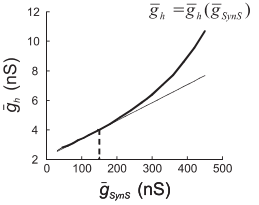
\includegraphics[width=1\linewidth]{Images/photo4_1.png}
\end{center}
  \end{minipage} 
  \begin{minipage}{0.4\linewidth}
  \begin{center}
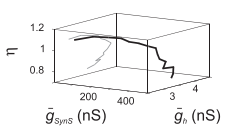
\includegraphics[width=1\linewidth]{Images/photo4_2.png}
\end{center}
  \end{minipage} 
  \caption{\textbf{Example of 1-dimensional level sets on the $\bar{g}_{h}-\bar{g}_{SynS}$  and $\bar{g}_{h}-\bar{g}_{SynS}-\eta$ parameter spaces.} Left: level set preserving the burst period (T) on the $\bar{g}_{h}-\bar{g}_{SynS}$ parameter space. Right: level set preserving both the burst period (T) and the intraburst spike frequency (f) on the $\bar{g}_{h}-\bar{g}_{SynS}-\eta$ parameter space. Figures taken from \cite{Oly}.}
  \label{photo4}
\end{figure}

On the other hand, the also look for level sets on the $\bar{g}_{h}-\bar{g}_{SynS}-\eta$ parameter space preserving both the burst period (T) and the intraburst spike frequency (f). Here, $\eta$ represents a scaling factor for the inactivation time constant $\tau_{h,CaS}$ of a slowly inactivating calcium low-threshold current $I_{CaS}$. Fig. (\ref{photo4})-Right shows an example of such an attribute level set.

Based on the implicit theorem, they also predict that if $m$ attributes are preserved on a given level set (computed with the algorithm proposed) in a $n$-dimensional parameter space, the level set has dimension $n-m$. 

\section{Compensatory mechanisms for level set generation}
In \cite{Rot}, they used two-dimensional neuron models with different level of complexity, to study the compensatory mechanisms leading to period and duty cycle (DC) level sets. DC is defined as the fraction of the period for which the oscillation is above half its amplitude.

Their work focus on exploiting mathematical phase plane analysis and $V$-speed diagrams to see differences between them along different points within the same attribute level set and, in this way, understand the compensatory mechanisms leading to the generation of attribute level sets.

As an example, Fig. (\ref{photo5})-Left shows period level sets on the $\lambda-\alpha$ parameter space on the FHN model. In addition, Fig. (\ref{photo5})- Middle shows $V-$ (red) and $w-$ (green) nullclines as well as the trajectories (blue) in the phase plane for two different points on a fixed period level set (normal and dashed lines), and Fig. (\ref{photo5})- Right shows the $V$-speed graph as a function of V for the same two points in the level set.

\begin{figure}[h]
\centering
        \begin{minipage}{0.33\linewidth}
            \begin{center}
                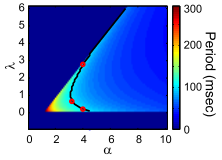
\includegraphics[width=1\linewidth]{Images/photo5_1.png}
            \end{center}
        \end{minipage} 
        \begin{minipage}{0.3\linewidth}
            \begin{center}
                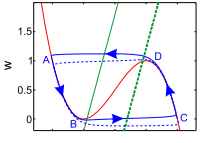
\includegraphics[width=1\linewidth]{Images/photo5_2.png}
            \end{center}
        \end{minipage} 
    \begin{minipage}{0.29\linewidth}
        \begin{center}
            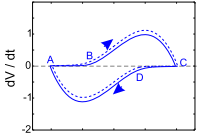
\includegraphics[width=1\linewidth]{Images/photo5_3.png}
        \end{center}
    \end{minipage} 
  
  \caption{\textbf{Period level sets on the $\lambda-\alpha$ parameter space, a phase-plane plot and a $V-$speed graph for the FHN model.} Left: period (T) level sets on the $\lambda-\alpha$ parameter space. Middle: an example of a phase-plane plot. Normal and dashed lines represent two different points within the same period level set. Red lines represents $V$-nullclines whereas green lines $w$-nullclines. Trajectories are in blue. Right: an example of a $V-$speed graph as a function of voltage $V$. Figures taken from \cite{Rot}.}
  \label{photo5}
\end{figure}

\section{Connecting cells within the same level set}
In \cite{Iii2019}, the ML model and a reduced two-dimesional conductance-based model (the Calcium/H -current oscillatory model) were used to form different homogeneous (identical cells) and heterogeneous (non-identical cells, but within the same level set) networks with electrical and chemical synapses. Significant differences between electrical and chemical networks in both models were found.

Cells were connected in a pairwise manner to produce different homogeneous and heterogeneous networks. Synaptic strength in networks was controlled by one parameters $G_{ElectSyn}$ and $G_{ChemSyn}$ in electrical and chemical networks respectively.

They show how electrical networks with different synaptic strength were able to preserve the individual cell frequency. In contrast, in synaptic networks they show either a decrease (Calcium/H -current model) or increase (ML model) in the individual cell frequency as the chemical synaptic strength increases.

Fig. (\ref{photo6}) shows the results in networks considering the Calcium/H -current model.

\begin{figure}[h]
\centering
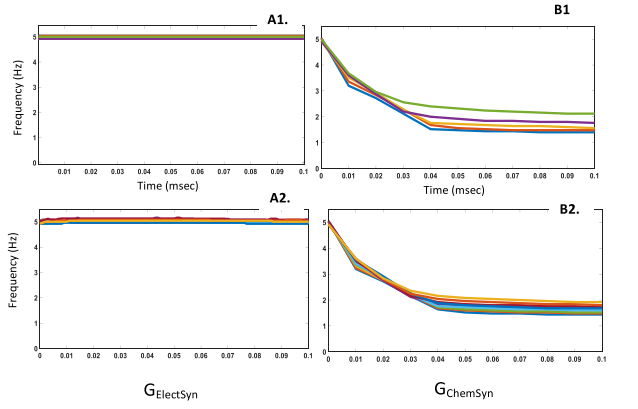
\includegraphics[width=0.8\linewidth]{Images/photo6_1.png}
  \caption{\textbf{Change in cell frequencies as per the increase in synaptic strengths.} A1-A2: electrical networks; B1-B2: chemical networks; A1-B1: homogeneous networks (identical cells); A2-B2: heterogeneous networks (cells within the same frequency level set). Figure taken from \cite{Iii2019}.}
  \label{photo6}
\end{figure}

Clearly, in chemical networks cells become part of a new network level set when connected. Regarding electrical networks, they show that electrical synapses was able to maintain the individual cell frequency, but other attributes, such as the amplitude, were not studied. Therefore, it is not known whether or not individual attribute level sets are preserved as well.

It is worth noting that, since different electrical synapses conductances preserve the network frequency, they constitute network frequency level sets on the connectivity parameter space. However, the connectivity parameter space considered here, as well as the network architecture, might be too simplified. 

Nevertheless, this work is a good starting point to the work developed in this project for two mainly reasons. Firstly, we ask if individual level sets are preserved when cells are electrically connected. Secondly, we would like to study more in detail network level sets on the connectivity parameter space in more complex networks architectures with higher dimensional parameter spaces. We will develop these ideas on a simplified mathematical network model.
